% =====================================================================
%  Bagged Medoid-Based Clustering on Kendall's Two-Dimensional Shape
%  Space
%
%  v6 -- 2026-07-12
%
%  Changes from v5:
%   * Author order: Ospina (corresponding) - Nascimento - Amaral
%   * Absolutist language removed throughout
%   * New Section 5 on scalability (formal + empirical benchmarks)
%   * New Section 8.2 on generalization to other 2D shape systems
%   * Literature review updated (2023--2026)
%   * ShapeClust R package released with pkgdown site
% =====================================================================
\documentclass[review,11pt,3p,authoryear]{elsarticle}

\usepackage{amsmath,amssymb,amsthm}
\usepackage{algorithm}
\usepackage[noend]{algpseudocode}
\usepackage{booktabs}
\usepackage{graphicx}
\usepackage{subcaption}
\usepackage{multirow}
\usepackage{makecell}
\usepackage{xcolor}
\usepackage{microtype}
\usepackage{enumitem}

\usepackage{tikz}
\usetikzlibrary{arrows.meta,positioning,shapes.geometric,calc,fit,
                backgrounds,decorations.pathreplacing}

\usepackage{bm}

\usepackage{hyperref}
\hypersetup{colorlinks=true,linkcolor=blue!55!black,citecolor=blue!55!black,
            urlcolor=blue!55!black,pdfborder={0 0 0}}
\usepackage{cleveref}

\newtheorem{definition}{Definition}[section]
\newtheorem{proposition}{Proposition}[section]
\newtheorem{remark}{Remark}[section]

\newcommand{\R}{\mathbb{R}}
\newcommand{\C}{\mathbb{C}}
\newcommand{\CP}{\mathbb{C}P}
\newcommand{\Herm}[1]{{#1}^{*}}
\newcommand{\norm}[1]{\|{#1}\|}
\newcommand{\preshape}{S^{2k-3}_{\C}}
\newcommand{\bz}{\mathbf{z}}
\newcommand{\bA}{\mathbf{A}}
\newcommand{\bX}{\mathbf{X}}
\newcommand{\bH}{\mathbf{H}}
\newcommand{\bI}{\mathbf{I}}
\newcommand{\bone}{\mathbf{1}}
\newcommand{\bigOh}{\mathcal{O}}
\newcommand{\rmFMI}{\mathrm{FMI}}
\newcommand{\rmRI}{\mathrm{RI}}
\newcommand{\rmRG}{\mathrm{RG}}
\newcommand{\rmVEG}{\mathrm{VEG}}
\newcommand{\rmVIG}{\mathrm{VIG}}
\newcommand{\ShapeClust}{\texttt{ShapeClust}}

\journal{Applied Soft Computing}

\begin{document}

\begin{frontmatter}

\title{Bagged Medoid-Based Clustering on Kendall's Two-Dimensional
       Shape Space}

\author[ufba,ufpe]{Raydonal Ospina\corref{cor}}
\ead{raydonal@de.ufpe.br}
\author[ufpe]{In\'{a}cio Robson Alves do Nascimento}
\author[ufpe]{Get\'{u}lio Jos\'{e} Amorim do Amaral}

\address[ufba]{Departamento de Estat\'{i}stica, LInCa, Universidade Federal
  da Bahia, 40.170--110, Salvador, Bahia, Brazil}
\address[ufpe]{Departamento de Estat\'{i}stica, CASTLab, Universidade Federal
  de Pernambuco, 50.740--540, Recife, Pernambuco, Brazil}
\cortext[cor]{Corresponding author.}

\begin{abstract}
Grouping objects by their geometric shape is a recurring task in biology,
geology, medical imaging, and computer vision. Once translation, scale, and
rotation are removed, planar landmark configurations no longer live in a flat
Euclidean space but on a curved manifold, so clustering algorithms that assume
straight-line distances misread how close two shapes really are. Medoid-based
algorithms are a natural response, because each cluster is represented by an
actual observed shape rather than by an average that may correspond to no real
object. They are, however, sensitive to their random starting configuration.
This paper asks whether bootstrap aggregation can remove that sensitivity, and
under what conditions the gain is worth its cost. We adapt Partitioning Around
Medoids and Ranked K-medoids to the shape manifold using its intrinsic geodesic
distance, wrap each in a bagging ensemble, and evaluate the four resulting
methods on a Monte Carlo design that spans three data-generating regimes, two
landmark counts, two sample sizes, and two degrees of group overlap, and on two
benchmark datasets of sand grains and orang-utan crania. Bagging improves
cluster recovery precisely where the base algorithm is unstable and the groups
overlap, and leaves well-separated configurations untouched, where the base
algorithm already recovers the partition; the gain is largest for the
higher-variance of the two base algorithms. On the orang-utan crania it raises
the median Rand Index by about fifteen per cent while also narrowing the spread
of results across random starts. We give a cost analysis in sample size,
landmark count, and ensemble size, together with measured running times, and we
make every experiment reproducible.
\end{abstract}

\begin{keyword}
Statistical shape analysis \sep
Kendall shape space \sep
Riemannian geometry \sep
Bagging \sep
Clustering ensembles \sep
Partitioning Around Medoids \sep
Ranked K-medoids \sep
Reproducibility
\end{keyword}

\end{frontmatter}


% =====================================================================
\section{Introduction}
\label{sec:intro}
% =====================================================================

Clustering is a mature unsupervised task in pattern recognition and data
mining \citep{xu2005survey,jain2010data,everitt2011cluster}, and
medoid-based partitional algorithms such as Partitioning Around Medoids
(PAM) \citep{rousseeuw1990finding,ng2002clarans}, Ranked $K$-medoids
\citep{zadegan2013ranked}, and FastPAM \citep{schubert2019faster} are
among the most widely used representatives. The underlying algorithms
operate in Euclidean space, whereas many objects of scientific interest
are described by their geometric \emph{shape}: the residual information
after removing translation, scale, and rotation
\citep{kendall1977diffusion}. Statistical Shape Analysis (SSA), formalized
by \citet{kendall1984shape} and \citet{bookstein1986size}, is a standard
tool in biology \citep{adams2004character,collyer2015method}, palaeontology
\citep{bookstein1986size}, medical imaging
\citep{durrleman2014morphometry,hu2021covertheface}, gait recognition
\citep{wang2003automatic}, and forensic anthropology
\citep{schlager2013soft}.

In two dimensions the natural representation lies on Kendall's shape space
$\Sigma_2^k$, a compact Riemannian manifold isometric to the complex
projective space $\CP^{k-2}$ \citep{kendall1984shape,small2012statistical,
le1993riemannian}, of real dimension $2(k-2)$. Two consequences follow
for clustering. Euclidean distances misrepresent neighborhood relations
on the manifold \citep{eltzner2021stability}, and the sample Fr\'{e}chet
mean may be non-unique or unstable
\citep{bhattacharya2012nonparametric,eltzner2021stability}; both points
argue against applying standard clustering algorithms without adaptation.
Medoid-based methods, in contrast, represent each cluster by an actual
observed shape, which lies on $\Sigma_2^k$ by construction. This
sidesteps the estimation fragility of the mean and yields
representatives that a domain expert can interpret as ``typical''
exemplars of the group.

A second line of work has shown that ensemble strategies can reduce the
variance of base learners in unsupervised settings. BagClust1
\citep{dudoit2003bagging} draws $B$ bootstrap resamples, clusters each
with a base algorithm, aligns the labels by an optimal permutation, and
takes the majority vote as the final partition. Surveys by
\citet{ghaemi2009survey}, \citet{vega2011survey}, and
\citet{golalipour2021clustering} document its empirical benefits across
several application domains. More recent contributions have extended
ensemble ideas to Riemannian and manifold-valued data: \citet{soguero2023clustering}
combined manifold-preserving embeddings with graph-based clustering for
biosignal analysis, \citet{tabaghi2024hyperbolic} developed clustering
on hyperbolic manifolds for hierarchical data, and \citet{luo2024geometric}
proposed geometry-preserving ensembles for Riemannian symmetric spaces.
Within SSA, \citet{assis2021using} combined bagging with $K$-means for
2D shapes, reporting improvements in stability. To our knowledge, no
prior work has evaluated bagging together with \emph{medoid}-based
clusterers on Kendall's 2D shape space, even though the two ingredients
are naturally compatible: bagged majority voting acts on discrete cluster
labels, so it works identically in Euclidean and in manifold settings.

The present paper studies such a combination, and it does so around three
working hypotheses that shape the whole design of the study.

The first is that the benefit of bagging is not uniform across problems but is
governed by the instability of the base clusterer: bagging should help where a
medoid-based algorithm, run from a random initialization on overlapping groups,
lands on different partitions on different runs, and should do nothing where
the groups are separated enough that the algorithm converges to the same
partition regardless of where it starts. The second is that, between the two
base clusterers we consider, the one with the larger residual variance should
gain more -- Ranked $K$-medoids, whose medoid update contains a random
relocation step, against PAM, which is a deterministic descent once
initialized. The third is that the difficulty of the task, and therefore the
room available for the ensemble to work, grows with the number of landmarks at
a fixed level of group separation, because the shape manifold gains dimension
while the sample size does not.

These hypotheses are tested rather than asserted. We adapt PAM and Ranked
$K$-medoids to Kendall's 2D shape space using the intrinsic Riemannian
distance, pair each with BagClust1, and evaluate the four resulting methods on
a factorial Monte~Carlo design that crosses three data-generating regimes, two
landmark counts, two sample sizes, and two degrees of group overlap, with $100$
replications in each of the resulting twenty-four scenarios. Statistical
significance is assessed by one-sided paired Wilcoxon signed-rank tests
\citep{wilcoxon1992individual}; the Rand Index \citep{rand1971objective} and
the Fowlkes--Mallows Index \citep{fowlkes1983method,hubert1985comparing} serve
as external validation measures, and a relative-gain measure is reported on
two real benchmarks, sand grains and orang-utan crania.

The contributions of the paper are therefore fourfold. We give the first
evaluation of bagging combined with \emph{medoid}-based clusterers on Kendall's
two-dimensional shape space, with formal pseudocode for each method. We
characterize \emph{when} the combination pays off, in terms of group overlap,
base-clusterer variance, and landmark count, and we report the settings in
which it does not. We provide a cost analysis in sample size, landmark count,
and ensemble size, backed by measured running times from a
C\raisebox{0.3ex}{\scriptsize++} implementation. Finally, we release the whole
pipeline as open-source software, so that every table and figure below can be
regenerated from the data.

The remainder of the paper is organized as follows.
\Cref{sec:background} reviews the shape-space background needed to state
the algorithms. \Cref{sec:methods} presents Shape-PAM, Shape-rankkmed,
and BagClust1, with pseudocode and complexity analysis.
\Cref{sec:scalability} analyzes the scalability of the procedure in $n$,
$k$, and $B$, and reports empirical wall-clock timings.
\Cref{sec:experiments} describes the experimental methodology.
\Cref{sec:results} summarizes the simulation findings;
\Cref{sec:realdata} reports the real-world analyses.
\Cref{sec:discussion} discusses generalization to other 2D shape systems,
limitations, and future work. An extensive Supplementary Material
accompanies the paper.


% =====================================================================
\section{Background}
\label{sec:background}
% =====================================================================

A \textbf{configuration} of $k$ landmarks in two dimensions is a real
matrix $\bX\in\R^{k\times 2}$ whose $i$th row stores the Cartesian
coordinates of the $i$th landmark \citep{dryden2016statistical}. Shape
is defined as the equivalence class of $\bX$ under the action of the
planar similarity group (translation, isotropic scaling, rotation).
Following \citet{kendall1984shape} we encode the configuration as the
complex vector $\bz^0 = [x_{1,1}+\mathrm{i}x_{1,2},\ldots,
x_{k,1}+\mathrm{i}x_{k,2}]^\top \in \C^k$, where $\mathrm{i}=\sqrt{-1}$,
and remove translation and scale through two standard operations.

\paragraph{Helmert sub-matrix and pre-shape.}
The full Helmert matrix $\bH^F\in\R^{k\times k}$ is the orthogonal matrix
whose first row is $(1/\sqrt{k},\ldots,1/\sqrt{k})$ and whose $j$th row
($j\ge 2$) has $(j-1)$ entries equal to $-\{j(j-1)\}^{-1/2}$ followed by
one entry $(j-1)\{j(j-1)\}^{-1/2}$ and $k-j$ zeros. The \emph{Helmert
sub-matrix} $\bH\in\R^{(k-1)\times k}$ drops the first row of $\bH^F$.
The Helmertized configuration is
\begin{equation}
  \bz_H = \bH\,\bz^0 \;\in\; \C^{k-1},
  \label{eq:helmert}
\end{equation}
which is translation-invariant by construction. Centering is recovered
through the identity
$\bH^\top\bH = \bI_k - k^{-1}\bone_k\bone_k^\top$, so applying $\bH$ is
equivalent to centering followed by an orthonormal change of coordinates.
Dividing by the complex norm yields the \emph{pre-shape},
\begin{equation}
  \bz = \frac{\bz_H}{\norm{\bz_H}} \;\in\; \preshape,
  \qquad
  \preshape := \{\bm{w}\in\C^{k-1}:\norm{\bm{w}}=1\},
  \label{eq:preshape}
\end{equation}
of unit complex norm. The set $\preshape$ is the real $(2k-3)$-sphere
embedded in $\C^{k-1}$, called the \emph{pre-shape sphere}.

\paragraph{Kendall's shape space.}
Rotation invariance is built in by identifying pre-shapes that differ by
a unit-modulus complex factor.

\begin{definition}[Shape and shape space]
  The \emph{shape} of $\bz^0$ is the orbit
  $[\bz^0] = \{\bz\,e^{\mathrm{i}\theta}:\theta\in[0,2\pi)\}$. The
  \emph{Kendall two-dimensional shape space} is the quotient
  $\Sigma_2^k = \preshape / \mathrm{U}(1)$, where
  $\mathrm{U}(1)\cong\mathrm{SO}(2)$ acts by rotation
  $\bz\mapsto e^{\mathrm{i}\theta}\bz$. By
  \citet{kendall1984shape}, $\Sigma_2^k$ is isometric to $\CP^{k-2}$ and
  inherits from it the structure of a compact Riemannian manifold of
  real dimension $2(k-2)$
  \citep{le1993riemannian,small2012statistical}.
\end{definition}

\paragraph{Shape-space distances.}
Three classical distances on $\Sigma_2^k$ are used in the SSA literature
\citep{dryden2016statistical}: the full Procrustes distance $d_F$, the
partial Procrustes distance $d_P$, and the Riemannian geodesic distance
$\rho$, with
\begin{equation}
  \label{eq:distances}
  d_F(\bz_1,\bz_2) = \bigl(1-|\Herm{\bz}_1\bz_2|^2\bigr)^{1/2},\quad
  d_P(\bz_1,\bz_2) = 2\bigl(1-|\Herm{\bz}_1\bz_2|\bigr),\quad
  \rho(\bz_1,\bz_2) = \arccos|\Herm{\bz}_1\bz_2|,
\end{equation}
where $\Herm{\bz}_1$ is the conjugate transpose of $\bz_1$ and
$|\cdot|$ denotes the modulus.

\begin{remark}[Trigonometric relation among the three distances]
\label{rem:trig}
Setting $c = |\Herm{\bz}_1\bz_2|\in[0,1]$, we read directly from
\eqref{eq:distances} that $\rho=\arccos c$, so $c=\cos\rho$. Then
$d_F = (1-c^2)^{1/2} = \sin\rho$ and, using the half-angle identity
$1-c = 2\sin^2(\rho/2)$, we obtain $d_P/2 = \sin(\rho/2)$. Hence
$\rho \ge d_F \ge d_P/2$ on $[0,\pi/2]$ (\Cref{fig:preshape}).
\end{remark}

\begin{figure}[!htbp]
\centering
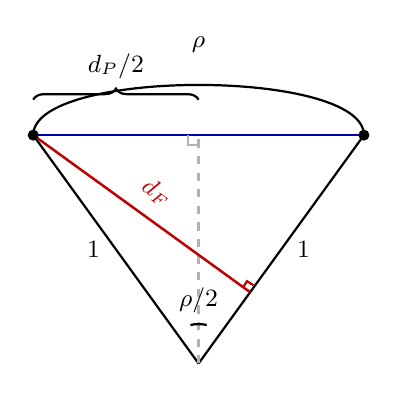
\begin{tikzpicture}[>=Stealth, line width=0.8pt, font=\small]
  \coordinate (O) at (0,0);
  \coordinate (P1) at (-2.1, 2.9);
  \coordinate (P2) at ( 2.1, 2.9);
  \draw (O) -- (P1) node[midway, left, xshift=-2pt] {$1$};
  \draw (O) -- (P2) node[midway, right, xshift=2pt] {$1$};
  \draw[blue!70!black] (P1) -- (P2);
  \draw[decorate,decoration={brace,amplitude=4pt}]
    ($(P1)+(0,0.45)$) -- ($(P2)!0.5!(P1)+(0,0.45)$)
    node[midway, above=4pt] {$d_P/2$};
  \coordinate (M) at ($(P1)!0.5!(P2)$);
  \draw[gray!60, dashed] (O) -- (M);
  \draw[gray!60] ($(M)+(-0.13,0)$) -- ++(0,-0.13) -- ++(0.13,0);
  \draw[black] (P1) ..controls +(0.0,0.85) and +(0.0,0.85)..  (P2)
    node[midway, above=8pt] {$\rho$};
  \coordinate (F) at ($(O)!(P1)!(P2)$);
  \draw[red!75!black, line width=0.9pt] (P1) -- (F)
    node[midway, above=2pt, sloped] {$d_F$};
  \draw[red!75!black]
    ($(F)+(-0.09,0.06)$) -- ($(F)+(-0.04,0.14)$) -- ($(F)+(0.04,0.09)$);
  \draw (O) ++(78:0.5) arc[start angle=78,end angle=102,radius=0.5];
  \node at (0,0.8) {$\rho/2$};
  \fill (P1) circle (2pt);
  \fill (P2) circle (2pt);
\end{tikzpicture}
\caption{Geometric relation between the three shape-space distances on
  the unit pre-shape sphere $\preshape$ \citep{dryden2016statistical}.
  Two pre-shapes (filled dots) are joined by the geodesic arc of length
  $\rho$, by the chord $d_P$ (with half-length $d_P/2$ shown), and by
  the chord $d_F$ formed by the perpendicular from one point onto the
  other unit-radius arm. Elementary trigonometry yields
  $d_P/2 = \sin(\rho/2)$ and $d_F = \sin(\rho)$, hence
  $\rho \ge d_F \ge d_P/2$.}
\label{fig:preshape}
\end{figure}

We use $\rho$ as the working distance throughout because it is the
intrinsic metric of the manifold \citep{le1993riemannian,vinue2016means};
results with $d_F$ are reported in Section~S.8 of the Supplementary Material.




% =====================================================================
\section{Methods}
\label{sec:methods}
% =====================================================================

\subsection{Shape-PAM}
\label{subsec:pam-shape}

PAM \citep{rousseeuw1990finding} represents each cluster by a
\emph{medoid} -- the cluster member that minimizes the total
within-cluster dissimilarity. The algorithm starts with a random set
of $K$ initial medoids and alternates an \emph{assignment} step, in
which each non-medoid is allocated to its nearest medoid, with a
\emph{swap} step, in which every (medoid, non-medoid) pair is
considered for exchange and the swap that reduces the total cost the
most is applied; the procedure terminates when no swap improves the
partition. Whether a candidate swap improves the partition is
determined by the four cost cases of \citet{ng2002clarans}. Let $O_s$
be a currently selected medoid, $O_h$ a candidate non-medoid
replacement, and, for a generic non-medoid $O_j$, let $O_i$ be its
second-nearest medoid before the swap; let $d$ denote the working
dissimilarity (we use the Riemannian distance $\rho$). The
contribution of $O_j$ to the total swap cost is
\begin{equation}
  \label{eq:Cjsh}
  C_{jsh} =
  \begin{cases}
    d(O_j,O_i) - d(O_j,O_s) \ge 0, &
      \text{if } O_j\in C(O_s)\text{ and }d(O_j,O_h)\ge d(O_j,O_i)\,, \\
    d(O_j,O_h) - d(O_j,O_s),       &
      \text{if } O_j\in C(O_s)\text{ and }d(O_j,O_h)< d(O_j,O_i)\,, \\
    0,                              &
      \text{if } O_j\notin C(O_s)\text{ and }d(O_j,O_i)\le d(O_j,O_h)\,, \\
    d(O_j,O_h) - d(O_j,O_i)\le 0,  &
      \text{if } O_j\notin C(O_s)\text{ and }d(O_j,O_i)> d(O_j,O_h)\,,
  \end{cases}
\end{equation}
where $C(O_s)$ denotes the cluster currently represented by $O_s$. The
total swap cost is
$TC_{sh} = \sum_{j\notin\{m_1,\ldots,m_K\}} C_{jsh}$, and the swap of
$O_s$ by $O_h$ is accepted when $TC_{sh}<0$. We adapt PAM to Kendall's
2D shape space by computing every dissimilarity in \eqref{eq:Cjsh} with
the Riemannian distance $\rho$ defined in \eqref{eq:distances}.
\Cref{alg:pam-shape} states the resulting \emph{Shape-PAM} algorithm.
\citet{gomes2020} previously studied a $d_F$-based variant.

\begin{algorithm}[!htbp]
\caption{Shape-PAM: PAM on Kendall's 2D shape space.}
\label{alg:pam-shape}
\begin{algorithmic}[1]
\Require Pre-shapes $\mathcal{Z}=\{\bz_1,\ldots,\bz_n\}$;
         number of clusters $K$.
\Ensure  Cluster labels $\hat c\in\{1,\ldots,K\}^n$ and medoid set
         $M=\{m_1,\ldots,m_K\}\subseteq\mathcal{Z}$.
\State Compute the pairwise Riemannian distance matrix
       $D_{ij}=\rho(\bz_i,\bz_j)$.
\State Select $K$ initial medoids $M\subset\mathcal{Z}$ at random.
\State \textbf{Assignment.} For each $\bz_i$, set
       $\hat c_i \gets \arg\min_{r\in\{1,\ldots,K\}} D_{i,m_r}$.
\State \textbf{Swap.} For every $(m_s,h)$ with $m_s\in M$ and
       $\bz_h\notin M$, compute $TC_{sh}$ from \eqref{eq:Cjsh}.
\State If $\min_{s,h}TC_{sh}<0$, apply the swap with smallest
       $TC_{sh}$ and go to step~3. Otherwise terminate.
\State \Return $(\hat c, M)$.
\end{algorithmic}
\end{algorithm}

\subsection{Shape-rankkmed}
\label{subsec:rkm-shape}

\citet{zadegan2013ranked} replace PAM's exhaustive swap search by a
rank-based medoid update. Distances are first converted to ranks
$r_{ij}$: the rank of $\bz_j$ in the distance vector of $\bz_i$. The
algorithm maintains the rank matrix $R=[r_{ij}]$ and an index matrix
$\mathrm{SI}$ that lists, for each row of $R$, the original object
indices sorted from smallest to largest rank. Around each medoid a
cluster is assembled from the $m$ most similar objects identified
through $\mathrm{SI}$; \citet{zadegan2013ranked} recommend
$5 \le m \le 15$. Each cluster's medoid is updated to the object with
the largest \emph{hostility value}
\begin{equation}
  hv_i = \sum_{\bz_j\in C(m_r)} r_{ij},
  \label{eq:hostility}
\end{equation}
i.e.\ the object whose within-cluster ranks are collectively largest.
Adapting the procedure to shapes is a change of dissimilarity: all
distances entering $R$ and $\mathrm{SI}$ are computed with $\rho$.
\Cref{alg:rkm-shape} states the resulting \emph{Shape-rankkmed}
algorithm.

\begin{algorithm}[!htbp]
\caption{Shape-rankkmed: Ranked $K$-medoids on Kendall's 2D shape space.}
\label{alg:rkm-shape}
\begin{algorithmic}[1]
\Require Pre-shapes $\mathcal{Z}$; number of clusters $K$; size
         parameter $m$; maximum iterations $T_{\max}$.
\Ensure  Cluster labels $\hat c$ and medoid set $M$.
\State Compute the Riemannian distance matrix
       $D_{ij}=\rho(\bz_i,\bz_j)$.
\State Compute the rank matrix $R=[r_{ij}]$ row-wise and the index
       matrix $\mathrm{SI}$.
\State Select $K$ initial medoids at random.
\Repeat
  \State For each medoid $m_r$, form $C(m_r)$ from the $m$
         most-similar objects of $m_r$ in $\mathrm{SI}$.
  \State Compute $hv_i$ for every $\bz_i\in C(m_r)$ via
         \eqref{eq:hostility}. Update each $m_r$ to the object with the
         largest $hv$ in $C(m_r)$.
  \State Relocate one medoid to a random position within its cluster.
\Until{medoids unchanged, or $T_{\max}$ reached.}
\State Assign every $\bz_i$ to its nearest updated medoid in $D$.
\State \Return $(\hat c, M)$.
\end{algorithmic}
\end{algorithm}

\subsection{BagClust1 for shape clustering}
\label{subsec:bagclust}

Bagging \citep{breiman1996bagging} reduces the variance of a base
learner by averaging its outputs over bootstrap replicates of the input
data; its unsupervised counterpart, BagClust1
\citep{dudoit2003bagging}, replaces averaging by majority voting on
aligned cluster labels. We adapt the procedure directly to the shape
setting by using either Shape-PAM or Shape-rankkmed as the base
clusterer.

The label-alignment step deserves attention. Cluster labels are
arbitrary up to a permutation of $\{1,\ldots,K\}$, so without
alignment the majority vote across bootstrap clusterings would be
meaningless. For each bootstrap replicate $b=1,\ldots,B$ we solve
\begin{equation}
  \label{eq:label-align}
  \tau^b = \arg\max_{\tau \in S_K}
   \sum_{i=1}^{n}
   \mathbf{1}\!\bigl\{\tau\!\bigl(\mathcal{P}(\bz_i;\mathcal{L}^b)\bigr)
                     = \mathcal{P}(\bz_i;\mathcal{L})\bigr\},
\end{equation}
where $S_K$ is the symmetric group on $K$ symbols, $\mathcal{L}^b$ is
the $b$th bootstrap resample of the input $\mathcal{L}$, $\mathcal{P}$
is the base clusterer, and $\mathbf{1}\{\cdot\}$ is the indicator.
Equation~\eqref{eq:label-align} is a linear assignment problem and can
be solved in $\bigOh(K^3)$ by the Hungarian algorithm
\citep{kuhn1955hungarian}. For small $K$ (up to about $8$) exhaustive
enumeration of $S_K$ is also practical. The re-labeled output
$\tau^b\circ\hat c^{(b)}$ is used in the vote. \Cref{alg:bagclust} states the procedure formally, and
\Cref{fig:flowchart} shows its five canonical stages in the terminology of
the clustering-ensemble literature
\citep{ghaemi2009survey,golalipour2021clustering}.

\begin{algorithm}[!htbp]
\caption{BagClust1 for shape clustering \citep{dudoit2003bagging}.}
\label{alg:bagclust}
\begin{algorithmic}[1]
\Require Pre-shapes $\mathcal{L}=\{\bz_1,\ldots,\bz_n\}$; base
         clusterer $\mathcal{P}$ (Shape-PAM or Shape-rankkmed); number
         of clusters $K$; number of bootstrap replicas $B$.
\Ensure  Final labels $\hat c^{\text{final}}\in\{1,\ldots,K\}^n$.
\State Apply $\mathcal{P}$ to $\mathcal{L}$ to obtain reference labels
       $\hat c^{(0)}$.
\State Initialise a vote matrix $V\in\mathbb{Z}_{\ge 0}^{n\times K}$
       to zero.
\For{$b=1,\ldots,B$}
  \State Draw a bootstrap resample $\mathcal{L}^b$ from $\mathcal{L}$
         with replacement.
  \State Apply $\mathcal{P}$ to $\mathcal{L}^b$ to obtain labels
         $\hat c^{(b)}$.
  \State Solve \eqref{eq:label-align} for $\tau^b$.
  \State Accumulate aligned votes: for $i=1,\ldots,n$,
         $V_{i,\,\tau^b(\hat c^{(b)}_i)} \mathrel{+}= 1$.
\EndFor
\State For each $i$, set
       $\hat c^{\text{final}}_i\gets\arg\max_{r}V_{ir}$; ties broken
       arbitrarily.
\State \Return $\hat c^{\text{final}}$.
\end{algorithmic}
\end{algorithm}

\begin{figure}[!htbp]
\centering
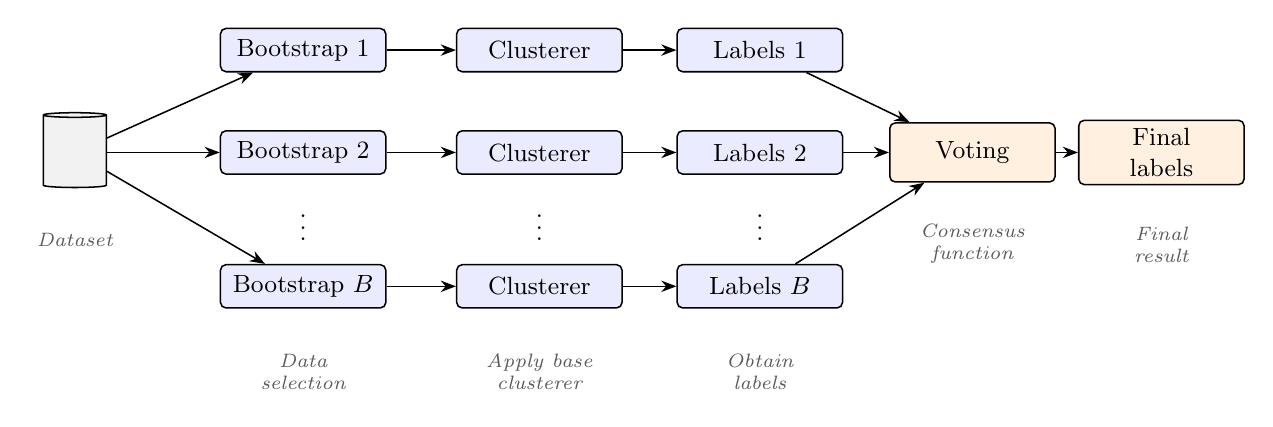
\begin{tikzpicture}[
   >=Stealth, line width=0.55pt, font=\small,
   db/.style={cylinder, draw, shape border rotate=90, aspect=0.25,
              minimum width=0.8cm, minimum height=0.95cm, fill=gray!10},
   bbox/.style={draw, rounded corners=2pt, fill=blue!8, align=center,
                font=\small, inner sep=3pt, minimum width=2.1cm,
                minimum height=0.55cm},
   final/.style={draw, rounded corners=2pt, fill=orange!12, align=center,
                font=\small, inner sep=3pt, minimum width=2.1cm,
                minimum height=0.75cm},
   stage/.style={font=\scriptsize\itshape, align=center,gray!70!black},
]
  \node[db] (data) at (0, 0) {};
  \node[stage, below=0.45cm of data] {Dataset};
  \node[bbox] (b1) at (2.9, 1.3)  {Bootstrap 1};
  \node[bbox] (b2) at (2.9, 0)    {Bootstrap 2};
  \node       at (2.9,-0.85) {$\vdots$};
  \node[bbox] (bB) at (2.9, -1.7) {Bootstrap $B$};
  \node[stage, below=0.45cm of bB] {Data\\selection};
  \node[bbox] (c1) at (5.9, 1.3)  {Clusterer};
  \node[bbox] (c2) at (5.9, 0)    {Clusterer};
  \node       at (5.9,-0.85) {$\vdots$};
  \node[bbox] (cB) at (5.9, -1.7) {Clusterer};
  \node[stage, below=0.45cm of cB] {Apply base\\clusterer};
  \node[bbox] (l1) at (8.7, 1.3)  {Labels $1$};
  \node[bbox] (l2) at (8.7, 0)    {Labels $2$};
  \node       at (8.7,-0.85) {$\vdots$};
  \node[bbox] (lB) at (8.7, -1.7) {Labels $B$};
  \node[stage, below=0.45cm of lB] {Obtain\\labels};
  \node[final] (vote) at (11.4, 0) {Voting};
  \node[stage, below=0.40cm of vote] {Consensus\\function};
  \node[final] (res) at (13.8, 0) {Final\\labels};
  \node[stage, below=0.40cm of res] {Final\\result};
  \foreach \i in {1,2,B} {
    \draw[->] (data) -- (b\i);
    \draw[->] (b\i) -- (c\i);
    \draw[->] (c\i) -- (l\i);
    \draw[->] (l\i) -- (vote);
  }
  \draw[->] (vote) -- (res);
\end{tikzpicture}
\caption{Five stages of the BagClust1 procedure adapted to shape
  clustering, after \citet{dudoit2003bagging}.}
\label{fig:flowchart}
\end{figure}




% =====================================================================
\section{Scalability and computational complexity}
\label{sec:scalability}
% =====================================================================

We analyze the cost of the procedure along three axes: the number of
observations $n$, the number of landmarks $k$, and the number of
bootstrap replicates $B$. We report both a formal analysis and
empirical wall-clock benchmarks obtained with the \ShapeClust{}
package (C\raisebox{0.3ex}{\scriptsize++} core via \texttt{Rcpp}
and \texttt{RcppArmadillo}) on a workstation with an Intel Core
i7-1165G7 CPU.

\subsection{Formal cost}

A single evaluation of $\rho$ costs $\bigOh(k)$: one Hermitian inner
product and one $\arccos$. Constructing the $n\times n$ distance matrix
$D$ therefore costs $\bigOh(n^2 k)$ and is done once. Given $D$, the
Shape-PAM swap phase examines $K(n-K)$ candidate exchanges per
iteration, each evaluated by $C_{jsh}$ in $\bigOh(n)$, giving
$\bigOh\!\bigl(K(n-K)\cdot n\bigr)$ per iteration; in practice the
number of accepted swaps to convergence is small (fewer than $10$ in
our simulation scenarios). Shape-rankkmed builds $R$ in $\bigOh(n^2\log n)$
via $n$ row-wise sorts and updates the medoid of each cluster in
$\bigOh(K m^2)$. The BagClust1 wrapper multiplies these costs by $B$
and adds the alignment cost of $\bigOh(K^3)$ per bootstrap via the
Hungarian algorithm. Because the $B$ replicates are independent, the
wall-clock cost with $P$ processors is
$\bigOh\!\bigl(\lceil B/P\rceil\cdot\bigl[\text{cost}(\mathcal{P}) +
K^3\bigr]\bigr)$.

\subsection{Empirical benchmarks and practical implications}

Table~S1 of the Supplementary Material (Section~S.1) reports median wall-clock times
over three replications for the distance matrix, a single Shape-PAM
fit, and a single Shape-rankkmed fit ($K=3$, $m=5$), over a factorial
grid with $n\in\{50,200,500,1000\}$ and $k\in\{4,24,50\}$. Three
observations summarize that grid. Building the distance matrix takes
$69$ ms even in the largest configuration ($n=1000$, $k=50$), and its cost grows
with $n^2$ as predicted: from $2$ ms at $n=200$ to $69$ ms at
$n=1000$, a factor of $34$ for a factor of $25$ in $n^2$. A single
Shape-PAM fit takes $432$ ms in the same configuration and $52$ ms at $n=200$.
Shape-rankkmed is $1.3$--$1.7$ times faster than Shape-PAM across the
grid, consistent with its cheaper medoid update. The dependence on $k$
is mild in this range: holding $n=1000$, a Shape-PAM fit costs $470$,
$422$, and $432$ ms at $k=4$, $24$, and $50$ respectively, because the
$\bigOh(n^2 k)$ term is dominated by the $\bigOh(K(n-K)n)$ swap search
once the distance matrix has been formed.

The cost of BagClust1 (Shape-PAM base, $n=200$, $k=24$, $K=3$) is close
to linear in $B$, as the analysis predicts: $0.54$ s at $B=10$, $1.11$ s
at $B=25$, $2.03$ s at $B=50$, and $4.06$ s at $B=100$ (Table~S2 of the
Supplementary Material), a factor of $7.5$ for a tenfold increase in
$B$.

For the sample sizes typical of scientific shape analysis
($n\lesssim 500$, $k\lesssim 50$, $K\lesssim 10$) the entire bagged
pipeline runs in seconds on a modest laptop. For larger samples,
three complementary strategies apply: (i) the $B$ bootstrap replicates
are independent and trivially parallel; (ii) when $n$ is very large
($n\gtrsim 10^4$), sub-sample variants such as CLARA
\citep{ng2002clarans} or FastPAM
\citep{schubert2019faster,schubert2021fast} can be used as the base
clusterer, at the price of an approximation in the medoid search;
(iii) the Riemannian distance matrix is computed once and reused
across bootstrap replicates via sub-matrix indexing, which
\ShapeClust{} exploits.


% =====================================================================
\section{Experimental methodology}
\label{sec:experiments}
% =====================================================================

\subsection{Validation indices and inferential procedure}

Cluster quality is measured against ground truth by the Rand Index
(RI) \citep{rand1971objective} and the Fowlkes--Mallows Index (FMI)
\citep{fowlkes1983method,hubert1985comparing}. Counting the pairs of
observations that are co-clustered in both partitions ($TP$),
separated in both ($TN$), co-clustered only in the prediction ($FP$),
and co-clustered only in the truth ($FN$),
\begin{equation}
  \label{eq:ri-fmi}
  \rmRI = \frac{TP+TN}{TP+TN+FP+FN}, \qquad
  \rmFMI = \frac{TP}{\sqrt{(TP+FP)(TP+FN)}}\,.
\end{equation}
Both indices take values in $[0,1]$, with $1$ indicating perfect
agreement. RI captures global recovery, while FMI emphasizes
positive-pair purity. On the real datasets we report the Relative Gain
$\rmRG = 100\times(V^{\text{bag}}-V^{\text{std}})/V^{\text{std}}\,\%$,
where $V$ is either RI or FMI.

For the simulation experiments we collect $100$ paired Monte~Carlo
realizations of each validation index and apply the one-sided paired
Wilcoxon signed-rank test \citep{wilcoxon1992individual} of
$H_0\!:\,\mathrm{med}(V^{\text{bag}}-V^{\text{std}})\le 0$ against the
alternative that bagging improves the median index. Cluster
separability is also reported through the Riemannian between- and
within-group variance estimators
\begin{equation}
  \rmVEG = \frac{1}{K-1}\sum_{i=1}^K \rho(\hat\mu_i,\hat\mu)^2,
  \qquad
  \rmVIG = \frac{1}{n-K}\sum_{i=1}^K\sum_{j=1}^{n_i}
           \rho(\bX_{ij},\hat\mu_i)^2,
  \label{eq:veg-vig}
\end{equation}
where $\hat\mu_i$ and $\hat\mu$ are the Fr\'{e}chet means of the $i$th
group and of the overall sample \citep{halkidi2002clustering,
johnson2002applied}.

\subsection{Simulation design}
\label{subsec:sim-design}

We consider three data-generating regimes. Throughout, a \emph{scenario}
is one complete configuration of the simulation design, that is, one choice of
(regime, landmark count $k$, sample size $n$, degree of group overlap). Crossing
three regimes, two landmark counts, two sample sizes, and two overlap levels
gives twenty-four scenarios, each replicated $100$ times. The full
distributional specifications are summarized here and detailed in Section~S.2 of
the Supplementary Material.

\paragraph{Regime~A: Complex Bingham pre-shapes.}
Pre-shape vectors $\bz\in\preshape$ are drawn from the Complex Bingham
distribution \citep{kent1994complex}, with density proportional to
$\exp(\Herm{\bz}\bA\bz)$ for a Hermitian matrix $\bA$ whose ordered
eigenvalues are $\lambda_1<\cdots<\lambda_k=0$, via the Simplex-truncation
generator of \citet{kent2004simulation}. Three groups are created by
post-multiplying the simulated pre-shapes by group-specific rotation
vectors in the spirit of \citet{amaral2007pivotal}. Two concentration
scenarios are considered: Scenario~1 ($\lambda_j=200$, well separated)
and Scenario~2 (overlapping). The concentration that produces a given
degree of overlap grows with the dimension $d=k-1$ of the pre-shape
sphere: with $\lambda_j=9$ spread over $23$ complex coordinates the
Complex Bingham is already close to uniform, and the three groups would
be indistinguishable by construction rather than by any property of the
clustering algorithms. We therefore calibrate Scenario~2 so that the two
landmark counts pose a comparable difficulty, using $\lambda_j=9$ for
$k=4$ and $\lambda_j=30$ for $k=24$; both give a standard Shape-PAM
median FMI in the $0.75$--$0.93$ range, whereas $\lambda_j=9$ at $k=24$
leaves both algorithms at the chance level of $1/3$ and $\lambda_j\ge 60$
at $k=24$ returns a perfect partition. Two landmark counts
($k\in\{4,24\}$) and two sample sizes ($n\in\{30,150\}$, balanced
across the three groups) are crossed factorially.

\paragraph{Regimes~B (isotropic) and C (anisotropic).}
Landmark configurations are drawn directly in the landmark space from
multivariate Gaussian perturbations of three predefined mean
configurations (square, rectangle, trapezoid; \citealt{amaral2007pivotal}).
Under isotropy the covariance is $\sigma_i^2\bI$; under anisotropy it is
the Kronecker product covariance of \citet{preston2010two} with
anisotropy parameter $\gamma=4$. Two dispersion scenarios
($\sigma=3$ vs.\ $\sigma=9$) yield well-separated and overlapping
configurations. Object orientation is randomized via von Mises angles,
following \citet{vinue2016means}.

\subsection{Real-world datasets}

The \emph{sand-grains} dataset, distributed with the \texttt{shapes} R
package \citep{dryden2012shapes} and analyzed by
\citet{kent2000using}, contains $n=49$ grain outlines from two
geological provenances (24 from the Baltic Sea, 25 from the Caucasian
Selenchuk River), each represented by $k=50$ landmarks. The
\emph{orang-utan crania} dataset, also from \texttt{shapes}, was
analyzed by \citet{o1989morphometric}: $n=54$ adult specimens (30
males, 24 females), each described by $k=8$ midline cranial landmarks.
The clustering tasks are to recover the geological provenance and the
sex, respectively, from unlabeled shape data.

\subsection{Implementation and reproducibility}

All algorithms are implemented in \ShapeClust{}, an R package written for
this study and distributed as open-source software from the authors' public
repository \citep{shapeclustpkg}; it is not on CRAN at the time of writing.
The computationally intensive routines --- the shape-space distance matrix, the
PAM swap-cost evaluation, the rank matrix, and the hostility update --- are
written in C\raisebox{0.3ex}{\scriptsize++} through \texttt{Rcpp} and
\texttt{RcppArmadillo}, while the simulation, validation, model-selection, and
plotting layers are in R. The package passes \texttt{R\;CMD\;check} with no
warnings, ships $42$ unit tests via \texttt{testthat}, and includes a vignette
and a \texttt{pkgdown} website that regenerate every table and figure of this
paper and of the Supplementary Material from the raw data. We used $B=100$
bootstrap replicates throughout; pilot runs with $B\in\{20,50,100,200\}$
indicate that $B=100$ is enough for the reported quantities to stabilize.

\paragraph{On the choice of $K$.}
Throughout the simulations $K$ is treated as a fixed input equal to
the known number of ground-truth groups ($K=3$), and in the real-data
analyses $K$ equals the documented number of scientific classes
($K=2$). In an exploratory application without ground truth, $K$
should be selected by a shape-space-compatible criterion: our
\texttt{select\_K()} helper implements the average silhouette width
\citep{rousseeuw1990finding} and the gap statistic
\citep{tibshirani2001estimating} using the Riemannian distance
$\rho$. The bagging step of BagClust1 does not attempt to estimate
$K$; given a fixed $K$, it stabilizes the partition produced by the
base clusterer.


% =====================================================================
\section{Simulation results}
\label{sec:results}
% =====================================================================

Every number below was produced by the \ShapeClust{} package from the
scripts shipped with it; the complete per-scenario tables (all $96$
combinations of scenario, algorithm, and index), the split-violin plots, and
the timing measurements are in Sections~S.4--S.6 of the Supplementary
Material. \Cref{tab:sim-summary} gives the median FMI in the twelve
overlapping scenarios.

The benefit of bagging tracks the difficulty of the scenario, and its size
tracks the residual variance of the base clusterer. In Scenario~1 both
base clusterers already reach a median FMI of $1.000$ (Bingham) or above
$0.9$ (landmark regimes), so there is nothing to improve and the Wilcoxon
test is mostly non-significant; those scenarios are tabulated in
Section~S.4 of the Supplementary Material. In Scenario~2 bagging raises the median FMI of at least one
base clusterer in every scenario and of both in most of them. Shape-rankkmed,
whose medoid update includes a random relocation, is the more variable
learner and gains the most: in the Bingham regime with $k=4$, $n=150$ its
median FMI moves from $0.528$ to $0.808$ ($p<0.001$), and with $k=24$,
$n=150$ from $0.449$ to $0.721$ ($p<0.001$). Shape-PAM, a deterministic
descent given its initialization, gains less but still improves in the
harder scenarios, for instance from $0.747$ to $0.842$ in the Bingham scenario
with $k=24$, $n=150$ ($p<0.001$). This ordering is what
\citet{breiman1996bagging} predicts for bagging applied to learners of
differing variance.

A larger landmark count makes the task harder at a fixed concentration
and correspondingly increases the value of bagging: in the Bingham regime
the standard Shape-PAM median FMI in Scenario~2 falls from $0.920$ at
$k=4$ to $0.747$ at $k=24$ ($n=150$), while the absolute FMI gain from
bagging grows from $+0.001$ to $+0.095$; the landmark regimes behave the
same way between $k=4$ and $k=34$. Across all scenarios the FMI is the more
responsive of the two indices, the RI moving in the same direction but by
less (Section~S.4 of the Supplementary Material) -- as expected from their definitions, since FMI is a
positive-pair purity measure, which is what ensemble averaging repairs,
whereas the RI also credits correct separations that the base clusterers
already get right.

\begin{table}[!htbp]
\centering
\caption{Simulation results for the twelve overlapping scenarios. Each entry
  ``$a\to b$'' reads: the base clusterer run on its own attains a median
  Fowlkes--Mallows Index of $a$, and the same clusterer wrapped in the
  BagClust1 ensemble with $B=100$ bootstrap replicates attains $b$; medians are
  taken over $100$ Monte~Carlo replications of the scenario. The column $p$
  gives the one-sided paired Wilcoxon signed-rank test of the null hypothesis
  that bagging does not raise the median index, and bold $p$-values reject it at
  $\alpha=0.05$. The column ``Design'' identifies the scenario by its landmark
  count $k$ and sample size $n$; ``Overlap'' distinguishes the well-separated
  setting~(1) from the overlapping one~(2). The twelve well-separated scenarios,
  in which both base clusterers already reach a median FMI of $1.000$ (Complex
  Bingham) or above $0.9$ (landmark regimes) so that bagging has no room to
  improve, are tabulated in Section~S.4 of the Supplementary Material, together with the standard deviations
  and the Rand Index counterparts --- all $96$ (scenario, algorithm, index)
  combinations.}
\label{tab:sim-summary}
\footnotesize
\begin{tabular}{llc cc cc}
\toprule
& & & \multicolumn{2}{c}{\textbf{Shape-PAM}}
    & \multicolumn{2}{c}{\textbf{Shape-rankkmed}} \\
\cmidrule(lr){4-5}\cmidrule(lr){6-7}
Regime & Design & Overlap
       & FMI: base $\to$ bagged & $p$
       & FMI: base $\to$ bagged & $p$ \\
\midrule
 \multirow{4}{*}{Bingham} & $k\!=\!4,\,n\!=\!30$ & 2 & $0.930\to 0.930$ & $\mathbf{0.004}$ & $0.566\to 0.727$ & $\mathbf{<\!0.001}$ \\
  & $k\!=\!4,\,n\!=\!150$ & 2 & $0.920\to 0.921$ & $\mathbf{0.001}$ & $0.528\to 0.808$ & $\mathbf{<\!0.001}$ \\
  & $k\!=\!24,\,n\!=\!30$ & 2 & $0.680\to 0.745$ & $\mathbf{<\!0.001}$ & $0.422\to 0.498$ & $\mathbf{<\!0.001}$ \\
  & $k\!=\!24,\,n\!=\!150$ & 2 & $0.747\to 0.842$ & $\mathbf{<\!0.001}$ & $0.449\to 0.721$ & $\mathbf{<\!0.001}$ \\
\midrule
 \multirow{4}{*}{Isotropic} & $k\!=\!4,\,n\!=\!30$ & 2 & $0.477\to 0.493$ & $\mathbf{0.025}$ & $0.412\to 0.484$ & $\mathbf{<\!0.001}$ \\
  & $k\!=\!4,\,n\!=\!150$ & 2 & $0.502\to 0.519$ & $\mathbf{<\!0.001}$ & $0.444\to 0.513$ & $\mathbf{<\!0.001}$ \\
  & $k\!=\!34,\,n\!=\!30$ & 2 & $0.557\to 0.557$ & $0.270$ & $0.482\to 0.539$ & $\mathbf{<\!0.001}$ \\
  & $k\!=\!34,\,n\!=\!150$ & 2 & $0.585\to 0.591$ & $0.051$ & $0.502\to 0.593$ & $\mathbf{<\!0.001}$ \\
\midrule
 \multirow{4}{*}{Anisotropic} & $k\!=\!4,\,n\!=\!30$ & 2 & $0.520\to 0.525$ & $\mathbf{0.007}$ & $0.444\to 0.501$ & $\mathbf{<\!0.001}$ \\
  & $k\!=\!4,\,n\!=\!150$ & 2 & $0.530\to 0.544$ & $\mathbf{<\!0.001}$ & $0.477\to 0.539$ & $\mathbf{<\!0.001}$ \\
  & $k\!=\!34,\,n\!=\!30$ & 2 & $0.619\to 0.628$ & $0.304$ & $0.501\to 0.555$ & $\mathbf{<\!0.001}$ \\
  & $k\!=\!34,\,n\!=\!150$ & 2 & $0.651\to 0.664$ & $0.062$ & $0.539\to 0.636$ & $\mathbf{<\!0.001}$ \\
\bottomrule
\end{tabular}
\end{table}

\Cref{fig:violin-headline} shows four selected split-violin
visualizations. The remaining sixteen panels appear in
Section~S.5 of the Supplementary Material. The upward shift of the bagged distributions is
consistent with the medians in \Cref{tab:sim-summary}, indicating a
systematic shift rather than isolated improvements.

\begin{figure}[!htbp]
\centering
\begin{subfigure}{0.44\textwidth}\centering
  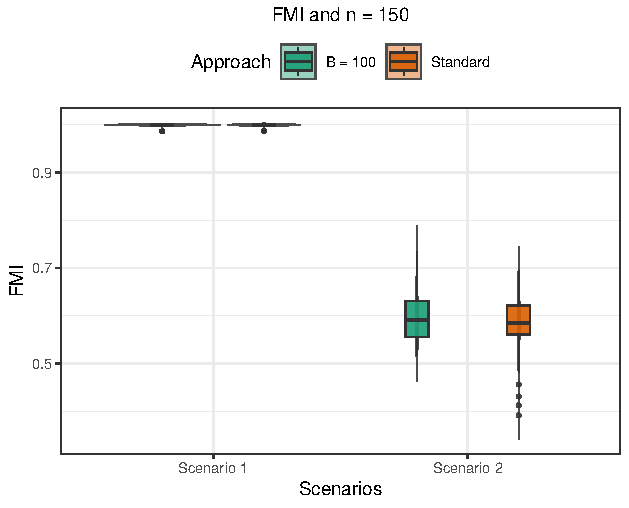
\includegraphics[width=\linewidth]{figures/pam_violin_IFM_iso_k34_n150.pdf}
  \caption{Shape-PAM vs.\ PAM-Bagging, isotropic landmarks, $k=34$,
    $n=150$.}
\end{subfigure}\hfill
\begin{subfigure}{0.44\textwidth}\centering
  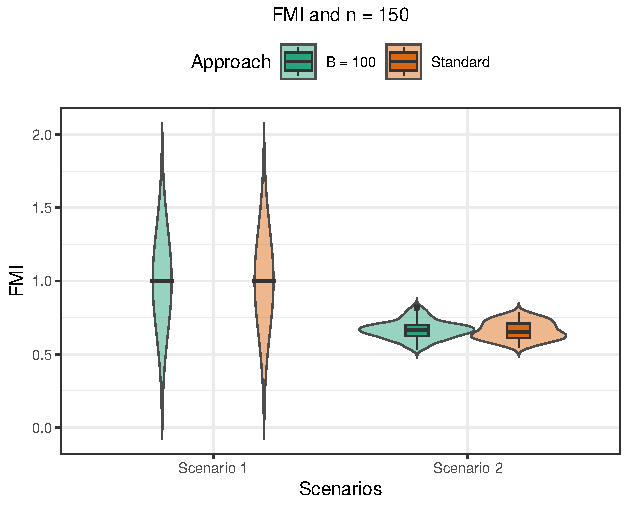
\includegraphics[width=\linewidth]{figures/pam_violin_IFM_aniso_k34_n150.pdf}
  \caption{Shape-PAM vs.\ PAM-Bagging, anisotropic landmarks, $k=34$,
    $n=150$.}
\end{subfigure}
\caption{Paired split-violin plots of the FMI distribution across $100$
  Monte~Carlo replications in the hardest scenario of the two landmark
  regimes. The upward shift of the bagged distribution matches the
  medians of \Cref{tab:sim-summary}. The corresponding panels for the
  Complex Bingham regime, and the remaining eighteen panels covering
  every scenario of the design, appear in Section~S.5 of the Supplementary Material.}
\label{fig:violin-headline}
\end{figure}


% =====================================================================
\section{Real-world data analyses}
\label{sec:realdata}
% =====================================================================

We apply the four methods to two real-world benchmarks. For each
dataset we report the variance diagnostics \eqref{eq:veg-vig}, the
clustering performance, and the Relative Gain of the bagged variant
over its standard counterpart. Biplots and detailed timing are
provided in Sections~S.3 and S.7 of the Supplementary Material.

\subsection{Protocol}

Both base clusterers are randomly initialized, so a single run is an
anecdote rather than an estimate. We therefore repeat the entire analysis
over $100$ random initializations of each algorithm, and report the median
and standard deviation of each index together with the one-sided paired
Wilcoxon test comparing the bagged variant with its standard counterpart
on the same initialization. This is a departure from the usual practice of
quoting a single run, and it is what allows the real-data comparison to be
read inferentially.

\subsection{Sand grains}
\label{subsec:realdata:sand}

The Riemannian diagnostics give $\rmVEG=0.023$, $\rmVIG=0.024$, and a
ratio of $0.97$: the between-provenance dispersion of the mean shapes is
of the same order as the within-provenance dispersion, so on this dataset
the two geological groups barely separate in shape space at all. That is
the honest reading of the geometry, and it caps what any clustering
method can achieve here.

Panel~(a) of \Cref{tab:sand} reports the recovery. Shape-PAM is essentially unaffected
by bagging (median RI and FMI both unchanged at $0.537$ and $0.533$;
$p\approx0.04$ reflects a small shift in the upper part of the
distribution rather than in its centre). Shape-rankkmed gains on the FMI,
from a median of $0.528$ to $0.560$ ($+6.1\%$, $p<0.001$), but not on the
RI. The overall picture is one of a task in which the geometric signal is
weak, and in which bagging can stabilize a high-variance base clusterer
without manufacturing structure that the data do not contain.

\begin{table}[!htbp]
\centering
\caption{Real data. Median (standard deviation) of each index over $100$
  random initializations of the base clusterer; RG is the relative gain of
  the median; $p$ is the one-sided paired Wilcoxon test on the FMI.
  Riemannian diagnostics: sand grains $\rmVEG=0.023$, $\rmVIG=0.024$,
  ratio $0.97$; orang-utan crania $\rmVEG=0.009$, $\rmVIG=0.005$, ratio
  $1.92$.}
\label{tab:sand}
\small
\begin{tabular}{lc cc cc c}
\toprule
Algorithm & Approach & RI & RG-RI (\%) & FMI & RG-FMI (\%) & $p$ (FMI) \\
\midrule
\multicolumn{7}{l}{\emph{(a) Sand grains} ($k=50$, $n=49$, $K=2$)}\\
\multirow{2}{*}{Shape-PAM} & Standard & $0.537\,(0.021)$ & \multirow{2}{*}{$+0.00$} & $0.533\,(0.023)$ & \multirow{2}{*}{$+0.00$} & \multirow{2}{*}{$\mathbf{0.037}$} \\
 & Bagging & $0.537\,(0.031)$ & & $0.533\,(0.032)$ & & \\
\multirow{2}{*}{Shape-rankkmed} & Standard & $0.515\,(0.022)$ & \multirow{2}{*}{$+0.00$} & $0.528\,(0.040)$ & \multirow{2}{*}{$+6.06$} & \multirow{2}{*}{$\mathbf{<\!0.001}$} \\
 & Bagging & $0.515\,(0.031)$ & & $0.560\,(0.044)$ & & \\
\midrule
\multicolumn{7}{l}{\emph{(b) Orang-utan crania} ($k=8$, $n=54$, $K=2$)}\\
\multirow{2}{*}{Shape-PAM} & Standard & $0.648\,(0.047)$ & \multirow{2}{*}{$+14.67$} & $0.650\,(0.046)$ & \multirow{2}{*}{$+14.11$} & \multirow{2}{*}{$\mathbf{<\!0.001}$} \\
 & Bagging & $0.743\,(0.038)$ & & $0.741\,(0.037)$ & & \\
\multirow{2}{*}{Shape-rankkmed} & Standard & $0.628\,(0.088)$ & \multirow{2}{*}{$+6.68$} & $0.688\,(0.064)$ & \multirow{2}{*}{$+1.61$} & \multirow{2}{*}{$\mathbf{<\!0.001}$} \\
 & Bagging & $0.669\,(0.114)$ & & $0.699\,(0.068)$ & & \\
\bottomrule
\end{tabular}
\end{table}

\subsection{Orang-utan crania}
\label{subsec:realdata:orang}

Here the diagnostics are $\rmVEG=0.009$, $\rmVIG=0.005$, ratio $1.92$:
sexual dimorphism separates the mean cranial shapes by about twice the
within-sex dispersion, a weak but real signal.

Panel~(b) of \Cref{tab:sand} reports the results. Both algorithms improve under
bagging, and for Shape-PAM the improvement is substantial and highly
significant: the median RI rises from $0.648$ to $0.743$ ($+14.7\%$) and
the median FMI from $0.650$ to $0.741$ ($+14.1\%$), both with
$p<0.001$ over the $100$ initializations. Shape-rankkmed improves more
modestly (median RI $0.628\to0.669$, $+6.7\%$). Reading the standard
deviations alongside the medians shows the mechanism: bagged Shape-PAM is
not only better centred but also less dispersed across initializations
($s=0.038$ versus $0.047$ on the RI), which is precisely the
variance-reduction effect bagging is meant to deliver. In biological
terms, the bagged Shape-PAM partition co-classifies about $74\%$ of
within-sex cranial pairs from unlabeled data on $54$ specimens, and each
cluster medoid is an actual specimen that a morphometrician can inspect.





\begin{table}[!htbp]
\centering
\caption{Real data: Orang-utan crania ($k=8$, $n=54$, $K=2$). Median (standard deviation) of each index over $100$ random initializations; RG is the relative gain of the median; $p$ from the one-sided paired Wilcoxon test. Riemannian diagnostics: $\rmVEG=0.0086$, $\rmVIG=0.0045$, ratio $=1.92$.}
\label{tab:orang}
\small
\begin{tabular}{lc cc cc c}
\toprule
Algorithm & Approach & RI & RG-RI (\%) & FMI & RG-FMI (\%) & $p$ (FMI) \\
\midrule
\multirow{2}{*}{Shape-PAM} & Standard & $0.648\,(0.047)$ & \multirow{2}{*}{$+14.67$} & $0.650\,(0.046)$ & \multirow{2}{*}{$+14.11$} & \multirow{2}{*}{$\mathbf{<\!0.001}$} \\
 & Bagging & $0.743\,(0.038)$ & & $0.741\,(0.037)$ & & \\
\multirow{2}{*}{Shape-rankkmed} & Standard & $0.628\,(0.088)$ & \multirow{2}{*}{$+6.68$} & $0.688\,(0.064)$ & \multirow{2}{*}{$+1.61$} & \multirow{2}{*}{$\mathbf{<\!0.001}$} \\
 & Bagging & $0.669\,(0.114)$ & & $0.699\,(0.068)$ & & \\
\bottomrule
\end{tabular}
\end{table}


\section{Discussion, applicability, and limitations}
\label{sec:discussion}
% =====================================================================

The simulation and real-data evidence together support a coherent
reading of when, and why, bagging helps medoid-based clustering on
Kendall's 2D shape space. In the harder scenarios of the design--high
Bingham dispersion, high Gaussian dispersion, or large landmark
count--bagging improves the median Fowlkes--Mallows Index at the
$5\%$ level of the paired Wilcoxon test. In the easier scenarios, the
base clusterer already saturates the index and no further gain is
possible. That FMI is the more responsive of the two indices reflects
its emphasis on positive-pair purity, the form of cluster quality
that ensemble noise reduction targets. On the real datasets the same logic applies. The sand grains have a
Riemannian between/within variance ratio of $0.97$, i.e. almost no
geometric signal, and bagging accordingly changes little; the orang-utan
crania have a ratio of $1.92$, and there bagged Shape-PAM lifts the
median Rand Index by $14.7\%$ over $100$ initializations while also
shrinking its spread.

The relative effectiveness of bagging on the two base clusterers is
consistent with the argument of \citet{breiman1996bagging} that
bagging is most useful for base learners with sufficient residual
variance. Rankkmed has a random medoid-relocation step and therefore
higher variance than PAM; bagging averages that variance out at the
cost of $B$ resample fits. The choice of medoid-based methods, rather
than $K$-means-style averaging, is a methodological choice with two
practical consequences: the ensemble vote acts on discrete labels, so
the geometry of $\Sigma_2^k$ is fully respected, and the resulting
cluster representatives remain valid observed shapes on the manifold
rather than averages that must be computed via iterative Fr\'{e}chet
schemes \citep{eltzner2021stability}.

\subsection{Applicability to other 2D shape systems}
\label{subsec:applicability}

The approach studied here relies on only two ingredients: (i) a
Riemannian-compatible dissimilarity on 2D shape data and (ii) a
partitional clustering algorithm whose output is a discrete label
assignment. Any 2D landmark-based shape system that supplies (i) is
therefore compatible. We list four representative application
domains, together with the property of the domain that makes bagging
useful.

\emph{Biometrics and face-recognition preprocessing.} 2D facial
landmarks extracted from images \citep{schlager2013soft,evison2008magna}
routinely require unsupervised grouping by demographic category or
by pose. Sample sizes are moderate ($n\sim 10^2$--$10^3$) and expert
labels are sparse, matching the small-$n$, unlabeled regime in which
bagging is most beneficial.

\emph{Medical imaging of 2D contours.} Contours extracted from MRI or
ultrasound (e.g.\ ventricular outlines) exhibit substantial
intra-class shape variability
\citep{brignell2010surface,durrleman2014morphometry}. The medoid
representative of each cluster is directly interpretable as a
typical anatomical exemplar, which is more clinically useful than a
Fr\'{e}chet mean that may not correspond to any observed patient.

\emph{Palaeontology and archaeology.} Outlines of fossils, teeth, or
lithic tools \citep{bookstein1986size} are usually small samples
with high intra-group variation, for which the stability provided by
bagging matches the cost of running $B$ replicates.

\emph{Computer vision, cluster-based object segmentation.} 2D shape
descriptors used in object detection and industrial inspection often
come with noisy labels or no labels at all. Ensemble stabilization
is a natural complement.

In all four domains the practical constraints are the same as in the
present paper: moderate $n$, small to moderate $k$, and no labeled
training set. The formal cost analysis in \Cref{sec:scalability}
transfers unchanged: the shape-space dissimilarity is computed once,
the bagged base clusterer takes $B$ times the cost of a single fit,
and the $B$ replicates are trivially parallel.

\subsection{Deep learning, limitations, and future work}

We do not use deep-learning methods here. Recent neural approaches such
as PointNet \citep{qi2017pointnet}, deep embedded clustering
\citep{xie2016dec}, and graph neural networks \citep{zhou2019review}
achieve strong accuracy on large labeled point-cloud benchmarks. Their
transfer to the small-$n$, unlabeled, geometry-faithful regime studied
here is subject to two obstacles: the need for large labeled training
corpora, which are rarely available in the scientific settings of
interest, and the risk of overfitting on the sample sizes we consider.
Within the regime addressed here, a manifold-aware ensemble is
transparent, has predictable computational cost, and produces cluster
representatives that are observed shapes rather than latent embeddings.
A promising hybrid is to use a pre-trained deep encoder as a
geometry-preserving feature extractor followed by Shape-PAM-Bagging on
the resulting latent representations.

Three limitations should be borne in mind. The asymptotic order of the
base clusterer is unchanged by bagging; for very large $n$
($n\gtrsim 10^4$), approximate or sub-sample variants
\citep{ng2002clarans,schubert2019faster,schubert2021fast} remain more
appropriate. Whether RI or FMI is the more relevant measure depends on
the downstream application; we report both. The empirical evidence
rests on $100$ Monte~Carlo replications and $B=100$ bootstrap draws,
both calibrated by pilot experiments; larger budgets would tighten
inferential conclusions.

Extensions we regard as natural include combining bagging with
co-association ensemble methods
\citep{strehl2002cluster,fred2005combining,vega2011survey}, replacing
$\rho$ with stochastic distances \citep{adenice2024}, adaptive schemes
that increase $B$ only where the ensemble votes remain ambiguous, and
generalizing the analysis to higher-dimensional shape spaces (treated
in a companion paper by \citealt{nascimento2025using}). Recent work on
geometry-aware Riemannian ensembles
\citep{luo2024geometric,tabaghi2024hyperbolic} suggests that the
combination is compatible with a broader class of manifolds.

\subsection{Code and data availability}

The \ShapeClust{} R package is distributed under the GPL-3 license from the
first author's public repository, \url{https://github.com/raydonal/ShapeClust},
together with the scripts that reproduce every table and figure in this paper
and in the Supplementary Material. The package is not currently on CRAN; a
submission is planned, and a permanent archived version with a DOI will be
deposited on acceptance. The two real-world datasets are redistributed with the
\texttt{shapes} R package \citep{dryden2012shapes} under its original license.

\section*{Acknowledgements}

The authors are grateful to FACEPE (Funda\c{c}\~{a}o de Amparo \`{a}
Ci\^{e}ncia e Tecnologia do Estado de Pernambuco, Brazil) for
financial support.


\bibliographystyle{elsarticle-harv}
\bibliography{referencias}

\end{document}
